\documentclass{ede}

\usepackage{lipsum}

\addbibresource{ref.bib}

\begin{document}

\edesetup{ Title={基于Django的留学生信息管理系统的设计与实现},%
  Author={葛宇航},%
  Address={西南林业大学~大数据与智能工程学院~昆明~650051},%
  Abstract={随着本校师资力量扩大,教育改革不断深化,使得留学生数量不断攀升,在日常学生管理
    工作当中,一个高效、方便、安全的平台显得十分尤为重要。本文基于Django这一Web开发框架,构
    建了了一个较为完善的留学生信息管理系统,实现的功能包括师生基本信息管理、班级管理、成绩
    录入与查询、考试管理等等,借助Django在Web开发中的强大优势,完善的ORM操作、丰富的功能模
    块、强大的数据处理、方便的url路由功能,快速高效地完成了项目开发,并上线使用。},%
  Keyword={Django;Python;留学生管理系统;B/S架构; MVT},%
  ztnum={99999999}, %中图分类号
  wxcode={88888888},%文献标识码
  enTitle={The design and implementation of a Django based oversea student information
    management system},%
  enAuthor={GE Yuhang},%
  enAddress={College of Big Data and Intelligence Engineering, Southwest Forestry
    University, Kunming 650224, Yunnan, China},%
  enAbstract={\lipsum[1]},%
  enKeyword={Python; Django; MIS},%
}

\twocolumn[
\begin{@twocolumnfalse}
  \maketitle
\end{@twocolumnfalse}
]

\section*{引言}

Web2.0时代,移动平台同时大为盛行,一个可适应多平台,并且能够快速进行开发的技术才能适应潮
流。Python是一个简单的、解释性、可交互、可移植、面向对象的高级编程语言,用于Web开发尤为合适,
它在软件开发、维护、调试、优化、部署等各个生命周期中都有十分高的效率。Django作为Python
Web开发中最为流行的应用框架,更是将Python的优势发挥到极致,它安装简单且灵活,使用方便,能够
开箱即用。遵循MVC开发模式,Django中内置了很多Web开发直接能使用的模块,同时集成了一个轻量级
的Webserver,能够方便地在本地进行调试。当下有许多著名的站点使用django进行开发,解释型语言开
发应用也越来越流行,基于Django这一高效框架,本文实现了一个功能较为完善的留学生信息管理系
统。

\section{关键技术介绍}

\subsection{Django框架}

Django\cite{nowamagic, 杨武帅2018基于}是Python中使用率最高的Web框架,它拥有良好的社区环境,
完善的版本迭代机制。遵循MVC的软件设计模式,用它可以快速、方便地开发出一个完整的Web应
用。Django框架的核心,如图\ref{fig:django}所示,包括一个轻量级的Web服务器,用于接受HTTP请求,
一个基于正则表达式的URL分发器,一个数据库模型用于建立数据模型与数据库相映射,一个视图系统用
于处理请求,以及一个模版系统。这种层次明晰的框架设计,在实际生产中极大地有利于应用软件的设
计与开发。

\begin{figure}%[h!]
  \centering
  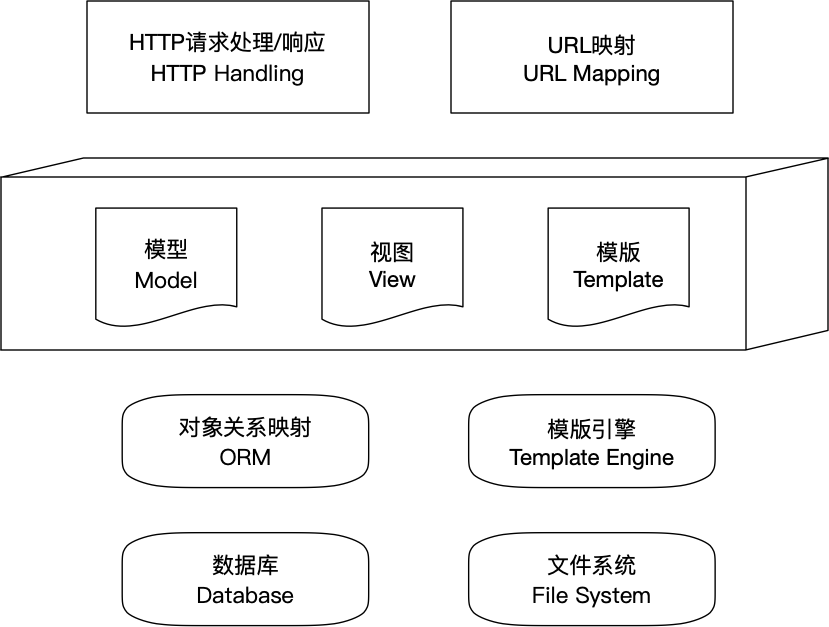
\includegraphics [width=.8\columnwidth]{./img/django}      
  \caption{Django架构总览图}\label{fig:django}
\end{figure}

\subsection{Django MVT}

Django的MTV设计模式(图\ref{fig:mvt})类似于标准的MVC, 包括四个模块:
\begin{enumerate}
\item Models.py用于创建数据库模型,是对数据库的上层封装,大大简化了编码过程中对数据库的增删
  改查操作,与MVC中的Model功能类似。
\item Views.py是主要的功能模块,负责业务逻辑处理,与Template进行数据交换,
  与MVC中的Control功能类似。
\item Templates文件夹中的保存的模版文件,用于生成最终HTML页面,与MVC中的View功能类似。
\item url.py则用于定义整个系统或某个子模块的路由表,指定了URL与views.py的映射关系。
\end{enumerate}
urls.py根据用户发起的请求,调用views.py中对应的函数,与数据模型以及模版进行交互,响应用户请
求。

\begin{figure}%[h!]
  \centering
  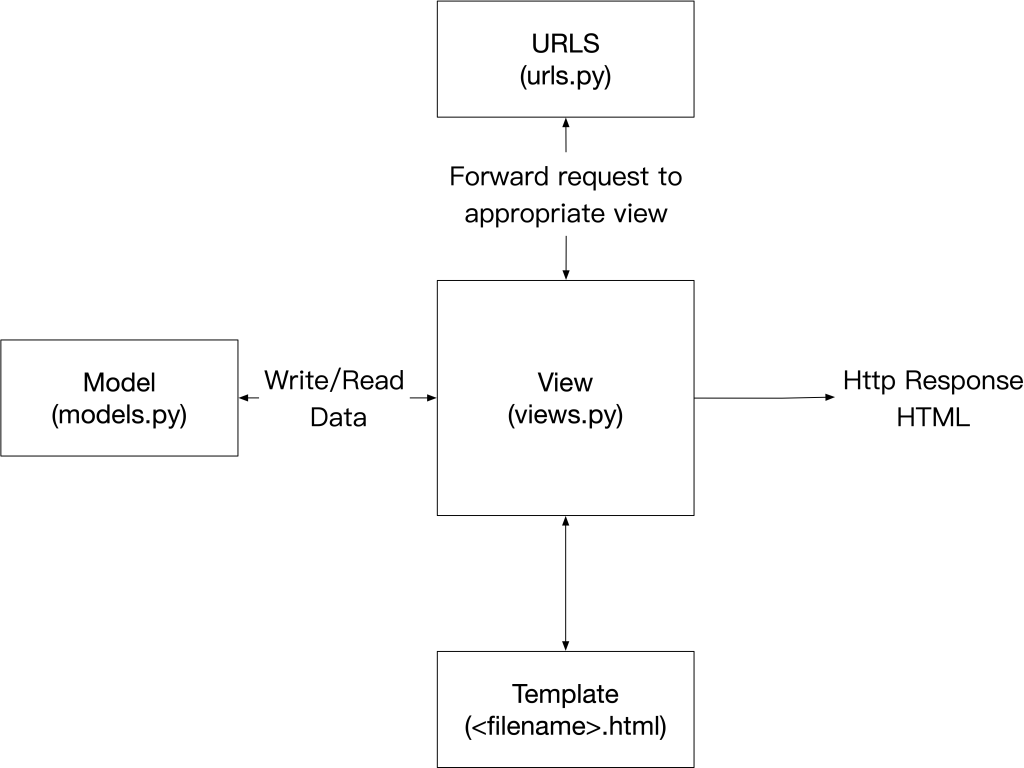
\includegraphics [width=.8\columnwidth]{./img/djangoMVT}      
  \caption{Django MVT}\label{fig:mvt}
\end{figure}

\subsection{Bootstrap}

Bootstrap\cite{汪红宇2017基于}是当下最流行的开源前端开发框架,有响应式布局、移动平台优先的
特性,为此十分适合本项目的前端构建。用户可以直接使用Bootstrap提供的CSS样式表,方便、快捷地
构建出自己想要的布局,更重要的是Bootstrap同时拥有大量的插件,设计开发的系统大部分业务需要进
行表格处理,Bootstrap table插件刚好可以满足系统的需求,bootstrap
table基于jquery\cite{Franklin2017Ajax}对表格处理的基本逻辑进行上层封装,开发者只需要对相应
的javascript代码进行简单的配置与参数传递,就可以完成单选、多选、排序、分页、编辑、过滤、导
入导出等常见功能,无需进行二次开发,大大减少的开发者的实际工作量。

\subsection{MySQL}

MySQL\cite{苟文博2017基于}有着高性能、成本低、可靠性好,在过去成为最流行的关系型数据
库。MySQL使用C和C++语言编写,具有可移植性,为包括Python在内的大量编程语言提供了API,Linux下
运行极为流畅,支持多线程。开源免费的特点使得其受到中小型企业的欢迎,它的这些优点,使其对于
本系统的开发尤为合适。

\section{系统架构分析}

本系统主要开发目的是以班级为单位的留学生个人信息、课程和成绩等信息的管理,增加工作效率,提
高管理能力。同时让学生可以更便捷地查询自己的成绩,本文吸取了大量相关学生信息管理系统开发的
经验,采用了B/S架构的设计思想,基于强大开源的Python的Web应用框架 Django进行二次开发,采
用 MVT 的软件设计模式,即模型 Model,视图 View 和模板 Template。使得维护起来较为方便,高内
聚低耦合。实现了相对完善的功能,其内容不仅涉及对学生资料进行管理分发,还包括对学生成绩信息,
考试信息,教师授课,成绩录入,综合评价等等,已投入实际使用,使得留学生管理工作趋于科学化、
高效化、规范化。

\section{系统架构设计分析}

\subsection{系统用户设计}

本系统面向的用户分为学生、教师、管理员等不同角色,每个角色权限与功能各不相同,用户输入用
户ID和密码,进行系统登录,后台通过用户ID对应的用户类型匹配返回的页面,实现角色分离。

\subsubsection{管理员}

管理员拥有最高的权限,包括班级管理、教师管理、课程管理、学生管理、考试管理、学生名单的导入
和学生成绩的导出(以班级为单位)等,管理员在考试管理页面考试科目相关设置,教师页面才能显示
出考试科目,完成考试后,对成绩进行录入。管理员也可以对成绩进行查询和统计等操作。

\subsubsection{教师}

教师对考试成绩的录入,点击对应考试最后一栏的成绩录入,即可获取参加该考试的所有学生,首先按
照平时、期中、期末分配成绩比例,然后再依次进行成绩录入,录入完成后,点击提交按钮即可保存,
此后提交按钮将变成无法点击状态,无法进行第二次提交操作。

\subsubsection{学生}

学生页面直接进行成绩查询,选择要查询的学年和学期,点击Search按钮,即可查询到自己的成绩数据。
当然,如果需要导出,也可通过工具栏上的导出工具进行成绩导出操作。

\subsection{主要功能模块}

如图\ref{fig:function}所示,系统的主要功能模块包括:
\begin{description}
\item [登录功能:] 系统入口,按角色进入不同页面,密码加密保存于数据库,登录时采用同样的加密
  算法,将用户输入的密码加密后与数据库比对,验证合法即可完成认证,成功跳转;
\item [角色管理:] 分为管理员,教师,学生等三个角色,便于控制用户各自权限;
  \begin{enumerate}
  \item 管理员: 拥有最大权限,班级管理,成绩管理,学生管理,教师管理,考试管理,考试成绩管
    理等,同时管理员可以给普通用户分配ID;
  \item 教师: 对考试成绩进行录入,查看与修改个人信息,管理学生信息,查看、统计学生成绩;
  \item 学生:对考试成绩进行查询,查看与修改个人信息;
  \end{enumerate}
\item [班级管理:] 添加、修改、删除班级基本信息,查看班级人员详情;
\item [教师管理:] 添加、修改、删除教师基本信息,分配教师工号,用于登录;
\item [课程管理:] 添加、修改、删除课程基本信息,安排任课教师并分配班级;
\item [考试管理:] 添加、修改、删除一场考试信息,设置考试时间、类型、科目、班级等;
\item [成绩管理:] 管理员对考试成绩进行修改和录入,不限次数,教师只能对考试成绩进行录入无法
  修改,且只能录入一次。
\end{description}

\begin{figure}%[h!]
  \centering
  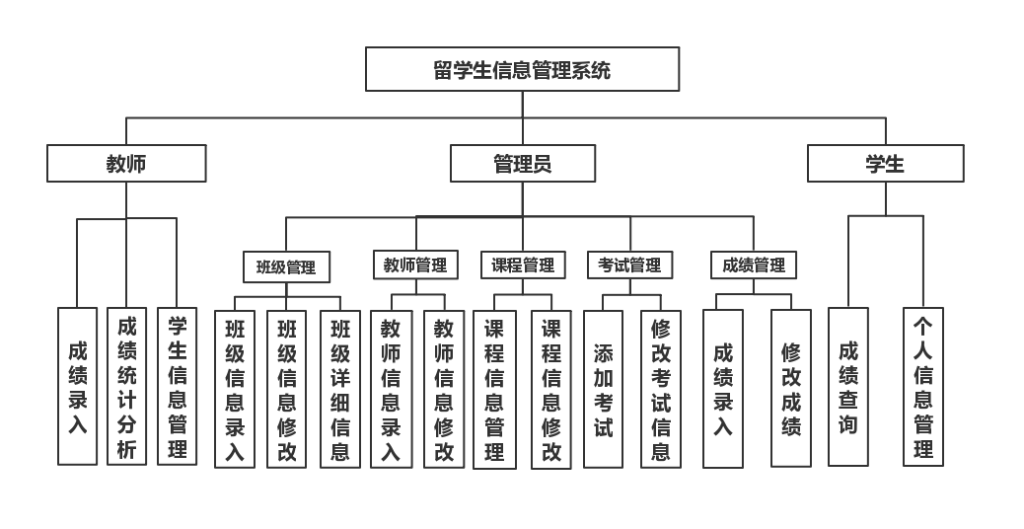
\includegraphics [width=.9\columnwidth]{./img/function}      
  \caption{系统功能模块设计图}\label{fig:function}
\end{figure}

\subsection{数据库连接}

本系统使用Mysql作为后台数据库,首先安装mysqlclient类库,作为django与mysql进行连接驱动,然后
在setting.py中配置数据库,以下是配置:

\begin{minted}{django}
DATABASES = {
  'default': {
     'ENGINE': 'django.db.backends.mysql',
     'NAME': 'studSys',
     'USER': 'root',
     'PASSWORD': '123456',
     'HOST': '127.0.0.1',
     'PORT': '3306',
  }
}
\end{minted}

还可以设置其他数据库, 如SqlServer, PostgreSQL, 只需修改数据库驱动ENGINE参数即可。配置后使
用python manager.py dbshell来测试是否连接成功。

根据数据库表结构创建相应的models.py,并将所属app添加入settings.py配置中。编写完成后使
用python manage.py validate 检查是否存在语法错误,若无语法错误,使用python manage.py
makemigrations 和 python manage.py migrate 迁移并同步数据库。

\subsection{前后端数据交互}

主要步骤:
\begin{enumerate}
\item 按照数据库设计,完成model.py模型文件编写(模型与数据库表一一映射,每个模型都是一个
  Python Class,每个模型类属性都相当于一个字段,model相当于提供一个访问数据库的API);
\item 将前端页面构建好,放入templates模版目录中;
\item 完成url的编写,对应即将使用的视图views文件;
\item 编写views文件,完成业务逻辑函数,渲染模版前端文件;
\end{enumerate}
下面以获取学生表数据为例分析代码:

\begin{minted}{django}
  urls.py:
  urlpatterns = [
    url(r'data', std.getData)
  ]
\end{minted}

前端发起查询的Ajax\cite{Liu2017Testing}请求,url路由通过匹配到视图下getData方法

\begin{minted}{django}
views.py:
@csrf_exempt
def getData(request):
'''获取数据'''
  if request.method == 'POST':
  '''ORM查询获取到所有的学生数据模型对象  
  Stud = StudTable.objects.all()
    dlen = len(Stud) 
    if Stud:
    '''遍历模型对象,获取具体数据'''
    for row in Stud:
      result = {}
      result['num'] = row.stuID_id 
      result['ch_name'] = row.stuChName
      ......
      jsonData.append(result)
  mydata = {
    "total": dlen,
    "rows": jsonData
  }
  return JsonResponse(mydata)
\end{minted}

定义数据长度dlen,使用一个数组jsonData来保存数据。getData方法判断为POST方法后,进行ORM查询
操作(StudTable.objects.all())从StudTable表中查询到所有的数据对象,遍历对象依次查询属性,
以字典的方式保存,再添加到jsonData中(目的是为了与bootstrap table的数据接口一致,代码块
中mydata即为标准数据接口,带total和rows两个属性,前者为数据长度,后者为实际传输的数据字典)。
获取到数据后再以json格式传回前端bootstrap table中,即可完成数据填充。

对学生数据的添加、删除、修改等操作的步骤类似,此处不做详细叙述。

\section{实现结果展示和分析}

\subsection{运行环境介绍}

\begin{enumerate}
\item 硬件环境。使用阿里巴巴提供的云服务器ECS;
\item 软件环境。操作系统是Debian GNU/Linux的Testing版。基于Linux的服务器平台相比Windows
  Server 更加稳定,也易于配置。使用Nginx做前端HTTP服务器,uWSGI作为中间件,通过它提供
  的API与后端Django应用通信,并与前端Nginx相链接;
\item 后台数据库。本系统采用mysql5.6作为数据库;
\item 系统结构。本系统采用B/S模式,客户端只需要一个浏览器就可以方便地使用,对用户硬件要求较
  低,可行性高;
\end{enumerate}

\subsection{主要界面展示}

下面是主要界面的展示,应文章篇幅原因,只展示部分页面,图\ref{fig:login}是登录界面,
图\ref{fig:admin}管理员登录,左边是可以操作的所有权限列表,包括班级管理、学生管理、教
师管理、课程管理、成绩管理等。

图\ref{fig:result}是管理员进行成绩管理的详情界面,可以进行包括筛选、修改、录入成绩等操作。
图\ref{fig:personal}是对学生个人信息进行管理的界面,可以直接通过行内编辑后自动保存新内容,
图\ref{fig:query}是学生端登录后查询成绩的页面。

\begin{figure}%[h!]
  \centering
  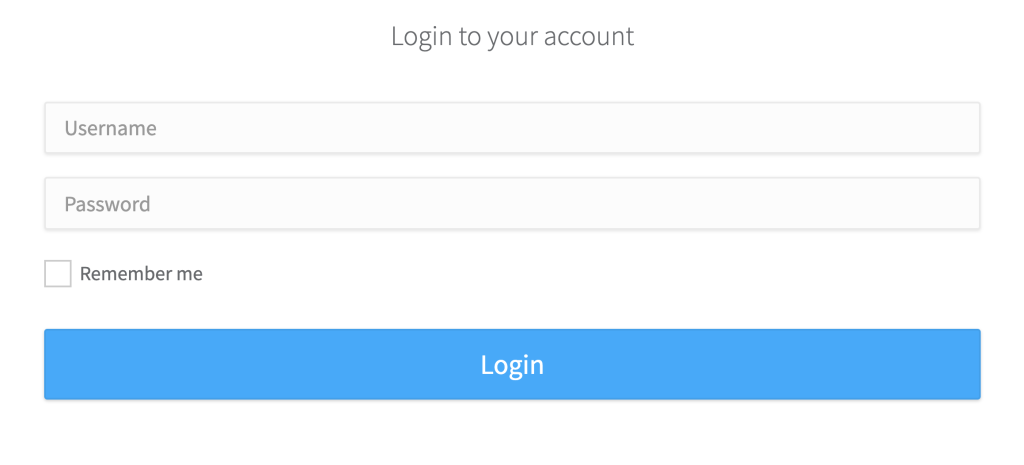
\includegraphics [width=.8\columnwidth]{./img/login}      
  \caption{登录页面}\label{fig:login}
\end{figure}

\begin{figure}%[h!]
  \centering
  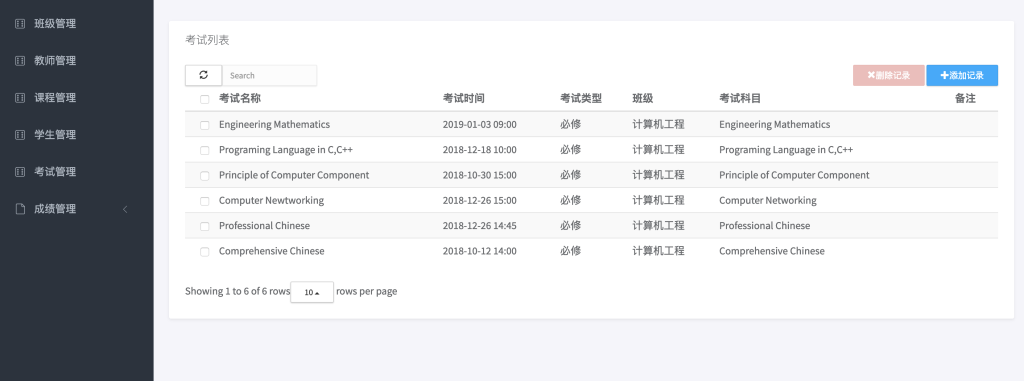
\includegraphics [width=.8\columnwidth]{./img/manager}    
  \caption{管理员界面}\label{fig:admin}
\end{figure}

\begin{figure}%[h!]
  \centering
  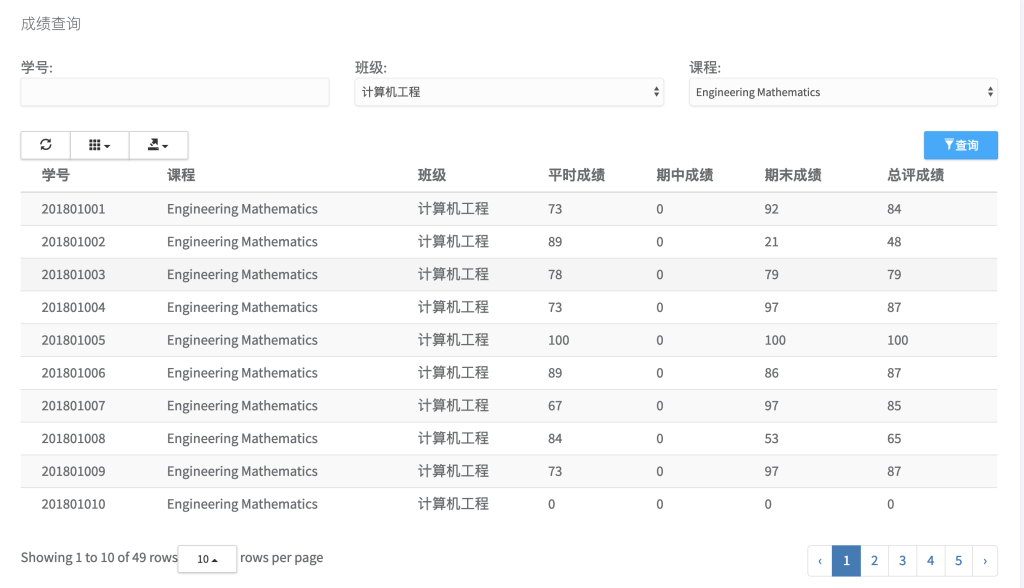
\includegraphics [width=.8\columnwidth]{./img/search}      
  \caption{管理员成绩管理}\label{fig:result}
\end{figure}

\begin{figure}%[h!]
  \centering
  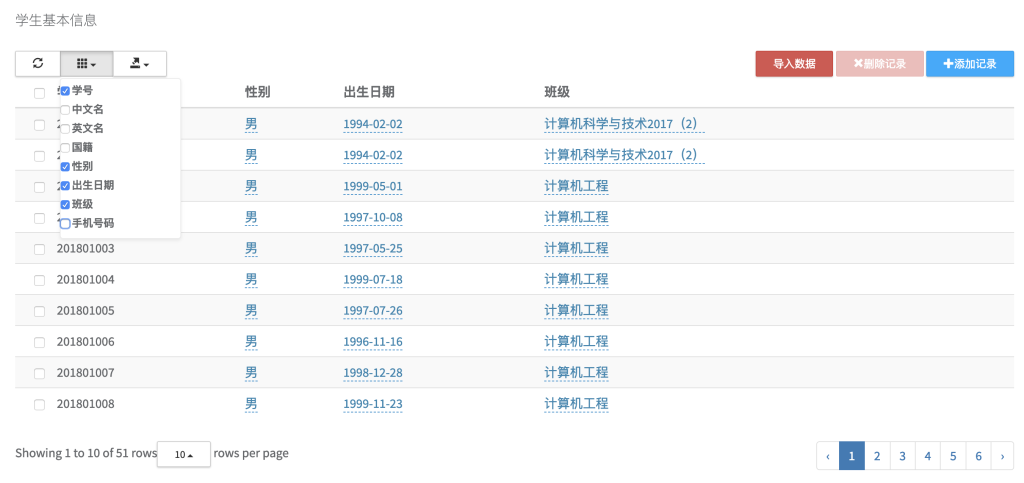
\includegraphics [width=.8\columnwidth]{./img/student}      
  \caption{学生信息管理}\label{fig:personal}
\end{figure}

\begin{figure}%[h!]
  \centering
  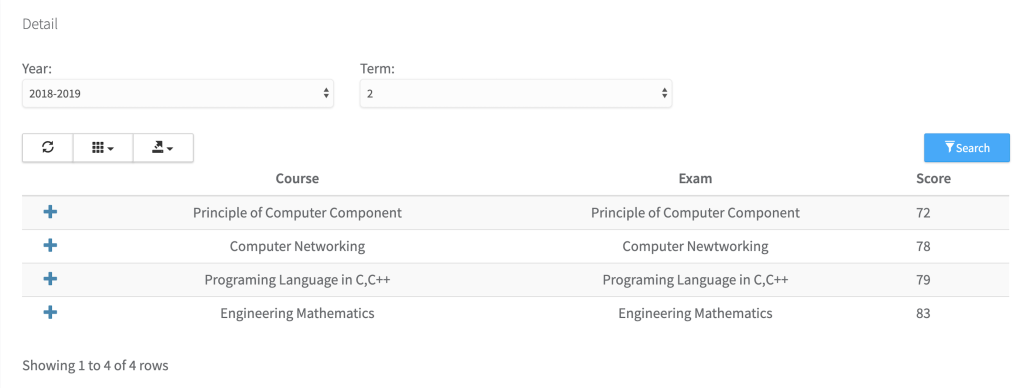
\includegraphics [width=.8\columnwidth]{./img/queryscore}      
  \caption{学生成绩查询}\label{fig:query}
\end{figure}

\section{结束语}

本系统主要解决了对留学生信息管理的问题,使得原本繁杂、重复、无序的工作变得更加有条理。系统
赋予不同角色相应的权限,增强了教师和教务管理的工作人员之间协同合作,信息共享更为方便快捷,
也使得学生能够更加方便的对自己的学习情况有更具体的了解。同时,该系统的实现体现
了Django在Web开发中的高效、敏捷等特点。

\makebib

\end{document}

%%% Local Variables:
%%% mode: latex
%%% TeX-master: t
%%% End:
